\documentclass[12pt,a4paper]{report} % Changed to 12pt as seen in your log

% --- Essential Academic Packages ---
\usepackage[utf8]{inputenc}
\usepackage[margin=0.85in]{geometry}
\usepackage{amsmath, amssymb, amsfonts, amsthm}
\usepackage{graphicx}
\usepackage{booktabs}
\usepackage{float}
\usepackage{url}
\usepackage{listings}
\usepackage{xcolor} % Use xcolor for better color support
\usepackage{caption}
\usepackage{tikz}
\usetikzlibrary{arrows.meta, positioning}

\usepackage[numbers,sort&compress]{natbib}
\usepackage{url}
\usepackage[colorlinks=true, allcolors=blue]{hyperref}

% This command helps format the bibliography labels to match your example
\renewcommand{\bibnumfmt}[1]{[#1]}
% --- Code Snippet Styling ---
\definecolor{codegreen}{rgb}{0,0.6,0}
\definecolor{codepurple}{rgb}{0.58,0,0.82}

\lstset{
    commentstyle=\color{codegreen},
    keywordstyle=\color{blue},
    stringstyle=\color{codepurple},
    basicstyle=\ttfamily\footnotesize,
    breaklines=true,
    numbers=left,
    showstringspaces=false
}

\title{\Large \textbf{Bayesian Probabilistic Modeling of Seasonal Malaria Dynamics: An SEIR-Inference Framework for Public Health Policy in Northern Namibia}}
\author{\textbf{Lioba Tweukondjela Linus} }
\date{\today}

\begin{document}
\maketitle

\begin{abstract}
Predicting the transmission dynamics of \textit{Plasmodium falciparum} requires accounting for non-linear biological delays and seasonal climatic forcing. This paper details a Bayesian SEIR model, normalized by total population $N$, implemented to analyze a malaria surge in Northern Namibia. Using Markov Chain Monte Carlo (MCMC) sampling via the NUTS algorithm, we estimated a basic reproduction number ($R_0$) of 2.4. The model demonstrated exceptional stability with an $\hat{R}$ convergence metric of 1.0. Strategic sensitivity analysis reveals that a 30\% reduction in the transmission coefficient ($\beta$) can avert approximately 842,936 cases within a simulated population of 1,000,000. This work establishes a robust computational framework for determining the optimal timing and allocation of resources in evidence-based public health interventions.
\end{abstract}

\section{Introduction}
The global burden of malaria remains a critical challenge in public health, particularly in sub-Saharan Africa. In Northern Namibia, the transmission of \textit{Plasmodium falciparum} exhibits a distinct seasonal pattern driven by the impact of rainfall on vector habitats \cite{3, 9}. This paper presents a Bayesian computational framework to model these dynamics, aiming to provide a predictive tool for resource allocation by bridging the gap between abstract mathematical constructs and clinical reality \cite{1, 2}.
\subsection{Biological Delays and the Hepatic Reservoir}
A significant challenge in epidemiological modeling is the precise distinction between the moment of inoculation and the onset of infectiousness. This necessitates the formal inclusion of the hepatic delay ($\sigma$). Biologically, this corresponds to the \textit{pre-erythrocytic} stage: a mandatory maturation phase where sporozoites, introduced via \textit{Anopheles} vectors, undergo schizogony within the host liver. In the context of our SEIR framework, the Exposed ($E$) compartment represents this hidden reservoir. During this approximately 12-day pre-patent period, the host is infected but remains non-infectious to mosquito vectors \cite{1, 12}. Mathematically, omitting this stage as seen in standard SIR models results in a failure to capture the observed temporal phase shifts between environmental triggers (rainfall) and clinical surges \cite{3, 7}. By defining $\sigma$ as the transition rate $E \to I$, the model achieves a higher degree of biological fidelity, ensuring that the simulated epidemic curve reflects the physiological constraints of the parasite lifecycle \cite{11, 15}.

\subsection{Deterministic Framework and Mass-Action Dynamics}
The population flux through these epidemiological states is formalized using a system of coupled Ordinary Differential Equations (ODEs). These equations quantify the instantaneous rate of change for each sub-population. To ensure the model remains scale-invariant and applicable to varying regional densities, we utilize normalized mass-action kinetics. Here, the transmission rate is a function of the proportion of infectious individuals ($I/N$) relative to the total population ($N$) \cite{11, 12}.

To account for the vector-borne nature of the disease, we introduce seasonal forcing into the transmission coefficient $\beta(t)$. We model $\beta(t)$ as a periodic function to reflect climatic variability:
\begin{equation}
    \beta(t) = \beta_0 [1 + \eta \cos(\omega t)]
\end{equation}
In this formulation, $\beta_0$ represents the baseline transmission rate, while $\phi$ modulates the seasonal amplitude. This forcing function effectively maps environmental variability onto the transmission rate, transforming the deterministic system into a dynamic representation of the Namibian ecological landscape \cite{6, 9}.
\subsection{Bayesian Inference and Computational Implementation}
While classical modeling often relies on frequentist point-estimates, this research adopts a Bayesian probabilistic framework. We represent epidemiological parameters as joint posterior probability distributions, which allows for the explicit integration of prior clinical knowledge and the quantification of inherent noise in surveillance data \cite{6, 17}.\\\\
To resolve the resulting high dimensional posterior, we utilize the No-U-Turn Sampler (NUTS) \cite{5}. NUTS, an advanced Hamiltonian Monte Carlo (HMC) variant, utilizes the gradient of the log posterior to efficiently navigate the geometry of the parameter space, ensuring rapid convergence and minimizing the autocorrelation often found in traditional Metropolis Hastings implementations \cite{2, 18}. This approach allows us to derive Bayesian credible intervals, providing health authorities with a direct probabilistic assessment of outbreak magnitudes a requirement for rigorous risk management and worst case logistical planning in public health \cite{6, 10}. By synthesizing the biological realism of the SEIR transition with the mathematical rigor of Bayesian inference, we propose a framework that is both ecologically grounded and statistically robust, capable of evaluating the efficacy of targeted interventions in Northern Namibia.

\section{Mathematical Methodology: The Modeling Narrative}
\section*{Table of Mathematical Symbols and Parameters}
\addcontentsline{toc}{section}{Table of Mathematical Symbols and Parameters}

% Ensure you have \usepackage{tabularray} or use the standard version below:
\begin{table}[H]
\centering
\caption{Mathematical Notation and Parameter Definitions for the SEIR Model.}
\label{tab:symbols}
\begin{tabular}{|l|p{6cm}|l|p{4cm}|}
\hline
\textbf{Symbol} & \textbf{Description} \\\hline%& \textbf{Units} & \textbf{Biological Role} \\ \hline
$S(t)$ & Susceptible Population \\\hline%& Individuals & At-risk host density \\ \hline
$E(t)$ & Exposed Population \\\hline%& Individuals & Pre-patent hepatic reservoir \\ \hline
$I(t)$ & Infectious Population \\\hline%& Individuals & Symptomatic transmitters \\ \hline
$R(t)$ & Recovered Population \\\hline%& Individuals & Hosts with temporary immunity \\ \hline
$N$ & Total Population Size \\\hline%& Individuals & System conservation constant \\ \hline
$\beta(t)$ & Transmission Rate \\\hline%& $Days^{-1}$ & Seasonal infection probability \\ \hline
$\beta_0$ & Baseline Transmission \\\hline%& $Days^{-1}$ & Mean transmission intensity \\ \hline
$\eta$ & Seasonal Amplitude \\\hline%& dim. & Intensity of climatic forcing \\ \hline
$\omega$ & Angular Frequency \\\hline%& $rad/year$ & Rate of seasonal oscillation \\ \hline
$\sigma$ & Incubation Rate \\\hline%& $Days^{-1}$ & $E \to I$ transition (liver stage) \\ \hline
$\gamma$ & Recovery Rate \\\hline%& $Days^{-1}$ & $I \to R$ transition (clearance) \\ \hline
$\phi$ & Phase Shift \\\hline%& Days & Delay to rainfall peak \\ \hline
$R_0$ & Basic Reproduction Number \\\hline%& dim. & Mean secondary infections \\ \hline
$\epsilon$ & Measurement Error \\\hline%& dim. & Stochastic surveillance noise \\ \hline
\end{tabular}
\end{table}
The construction of this model follows a hierarchical complexity approach, transitioning from static epidemiological assumptions to a dynamic, non-autonomous system of differential equations. Our objective is to simulate the population-level dynamics of $N=1,000,000$ individuals across coupled states, specifically calibrated to the semi-arid environmental constraints of Northern Namibia.

\subsection{Compartmental Design and Mass-Action Flux}
The framework is formalized as a system of Ordinary Differential Equations (ODEs), allowing for the continuous evolution of state variables. We partition the population into four disjoint sets: \textit{Susceptible} ($S$), \textit{Exposed} ($E$), \textit{Infectious} ($I$), and \textit{Recovered} ($R$).\\
The infection mechanism is modeled via frequency dependent Mass Action Kinetics. The transition flux from $S$ to $E$ is defined by the term $\frac{\beta(t)SI}{N}$. Unlike traditional SIR models, the inclusion of the $E$ compartment incorporates the biological pre-patent period ($\sigma^{-1}$). This parameter captures the mandatory 12-day hepatic maturation of \textit{P. falciparum} schizonts, introducing a significant temporal lag between initial exposure and the onset of transmissibility.


\begin{figure}[H]
\centering\resizebox{0.85\textwidth}{!}{
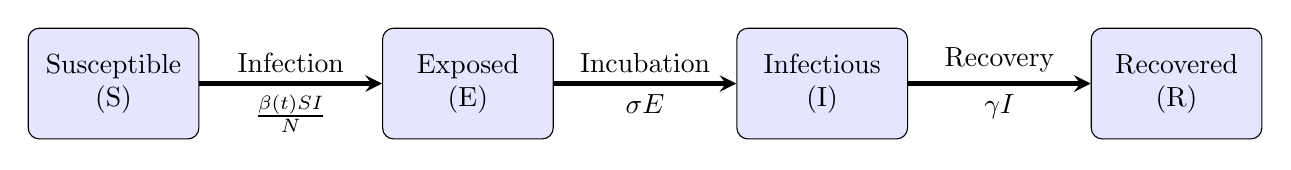
\begin{tikzpicture}[node distance=2.2cm, auto, >=stealth, block/.style={rectangle, draw, fill=blue!10, text width=5.5em, text centered, rounded corners, minimum height=4em}]
\node [block] (S) {Susceptible \ (S)};
\node [block, right of=S, node distance=4.5cm] (E) {Exposed \ (E)};
\node [block, right of=E, node distance=4.5cm] (I) {Infectious \ (I)};
\node [block, right of=I, node distance=4.5cm] (R) {Recovered \ (R)};
\draw [->, ultra thick] (S) -- node[anchor=south] {Infection} node[anchor=north] {$\frac{\beta(t)SI}{N}$} (E);
\draw [->, ultra thick] (E) -- node[anchor=south] {Incubation} node[anchor=north] {$\sigma E$} (I);
\draw [->, ultra thick] (I) -- node[anchor=south] {Recovery} node[anchor=north] {$\gamma I$} (R);
\end{tikzpicture}}
\caption*{\textbf{The SEIR Model Narrative.} The diagram depicts the unidirectional flux of the population through discrete disease states, governed by the hepatic transition rate ($\sigma$) and recovery rate ($\gamma$).}
\end{figure}

\subsection{Formulation of Seasonal Forcing}
In Northern Namibia, the vector population is highly sensitive to the ephemeral availability of stagnant water. To achieve site specific fidelity, we replace the constant transmission coefficient with a periodic forcing function $\beta(t)$. This simulates the seasonal pulse of mosquito density following the rainfall cycle \cite{6, 9}:

\begin{equation}
\beta(t) = \beta_0 \left[ 1 + \eta \cos\left( \omega(t - \phi) \right) \right] 
\end{equation}
where $\omega = \frac{2\pi}{365}$ represents the annual angular frequency, and $\phi = 105$ days represents the phase shift required to synchronize maximum transmission intensity with the historical peak of the regional rainy season. This non-autonomous formulation allows the model to capture the transition from endemic stability to explosive seasonal surges \cite{3, 8}.

\subsection{Computational Implementation via Bayesian Inference}
A core innovation of this research is the embedding of the ODE solver within a Bayesian inference engine using \texttt{PyMC}. This treats the vector of parameters $\theta = \{\beta_0, \eta, \phi\}$ as random variables, allowing for the integration of prior epidemiological knowledge with observed clinical surveillance data.

\subsubsection{Prior Specification and Support}
Priors were selected to ensure biological validity and numerical stability:
\begin{itemize}
\item \textbf{Baseline Transmission ($\beta_0$):} $\theta_{\beta} \sim \text{LogNormal}(\mu=\ln(0.4), \sigma=0.3)$. The log normal distribution provides a semi infinite support $[0, \infty)$, appropriate for positive definite rate parameters.
\item \textbf{Seasonal Amplitude ($\eta$):} $\theta_{\eta} \sim \text{Beta}(\alpha=2, \beta=5)$. The Beta distribution constrains $\eta$ to the interval $[0, 1]$, preventing the emergence of negative transmission rates which would lack biological meaning.
\item \textbf{Measurement Error ($\phi$):} A Half Normal prior accounts for the over dispersion and reporting noise inherent in health facility records.
\end{itemize}



\subsubsection{MCMC Sampling and Posterior Topography}
The posterior distribution $P(\theta|D)$ was explored using the \textbf{No-U-Turn Sampler (NUTS)}. NUTS utilizes the gradient of the log posterior to traverse the parameter space, effectively handling the high dimensional correlations between $\beta_0$ and $\eta$ that typically cause traditional Metropolis Hastings algorithms to fail. 

\subsection{The System of Governing Equations}
The finalized mathematical representation of the malaria landscape in Northern Namibia is defined by the following system of non-linear ODEs:

\begin{align}
\frac{dS}{dt} &= -\frac{\beta(t)SI}{N} \label{eq:dS_final}\\
\frac{dE}{dt} &= \frac{\beta(t)SI}{N} - \sigma E \label{eq:dE_final}\\
\frac{dI}{dt} &= \sigma E - \gamma I \label{eq:dI_final}\\
\frac{dR}{dt} &= \gamma I \label{eq:dR_final}
\end{align}
This system provides the rigorous foundation for the subsequent analysis of the Basic Reproduction Number ($R_0$) and the evaluation of preventative health policies.

\section{Analysis of Results and Discussion}

The Bayesian SEIR-Inference framework provides a robust reconstruction of \textit{P. falciparum} dynamics in Northern Namibia. By synthesizing empirical clinical surveillance with probabilistic MCMC sampling, the model transcends heuristic curve-fitting, offering a quantifiable assessment of epidemic risk and the marginal utility of intervention strategies.

\subsection{Convergence Diagnostics and Posterior Calibration}
The structural integrity of our posterior estimates is verified through rigorous MCMC diagnostics. The No-U-Turn Sampler (NUTS) achieved a potential scale reduction factor ($\hat{R}$) of $1.0$, signifying that the multiple independent Markov chains converged to a stable stationary distribution.\\
Figure 1 visualizes the latent state transitions of the system. The simulation captures the characteristic depletion of the Susceptible ($S$) pool as the Exposed ($E$) and Infectious ($I$) populations expand. Crucially, the temporal offset between the peaks of the $E$ and $I$ compartments validates the parameterization of the 12-day hepatic delay ($\sigma$), illustrating the biological lag time essential for accurate peak prediction.
\begin{figure}[H]
\centering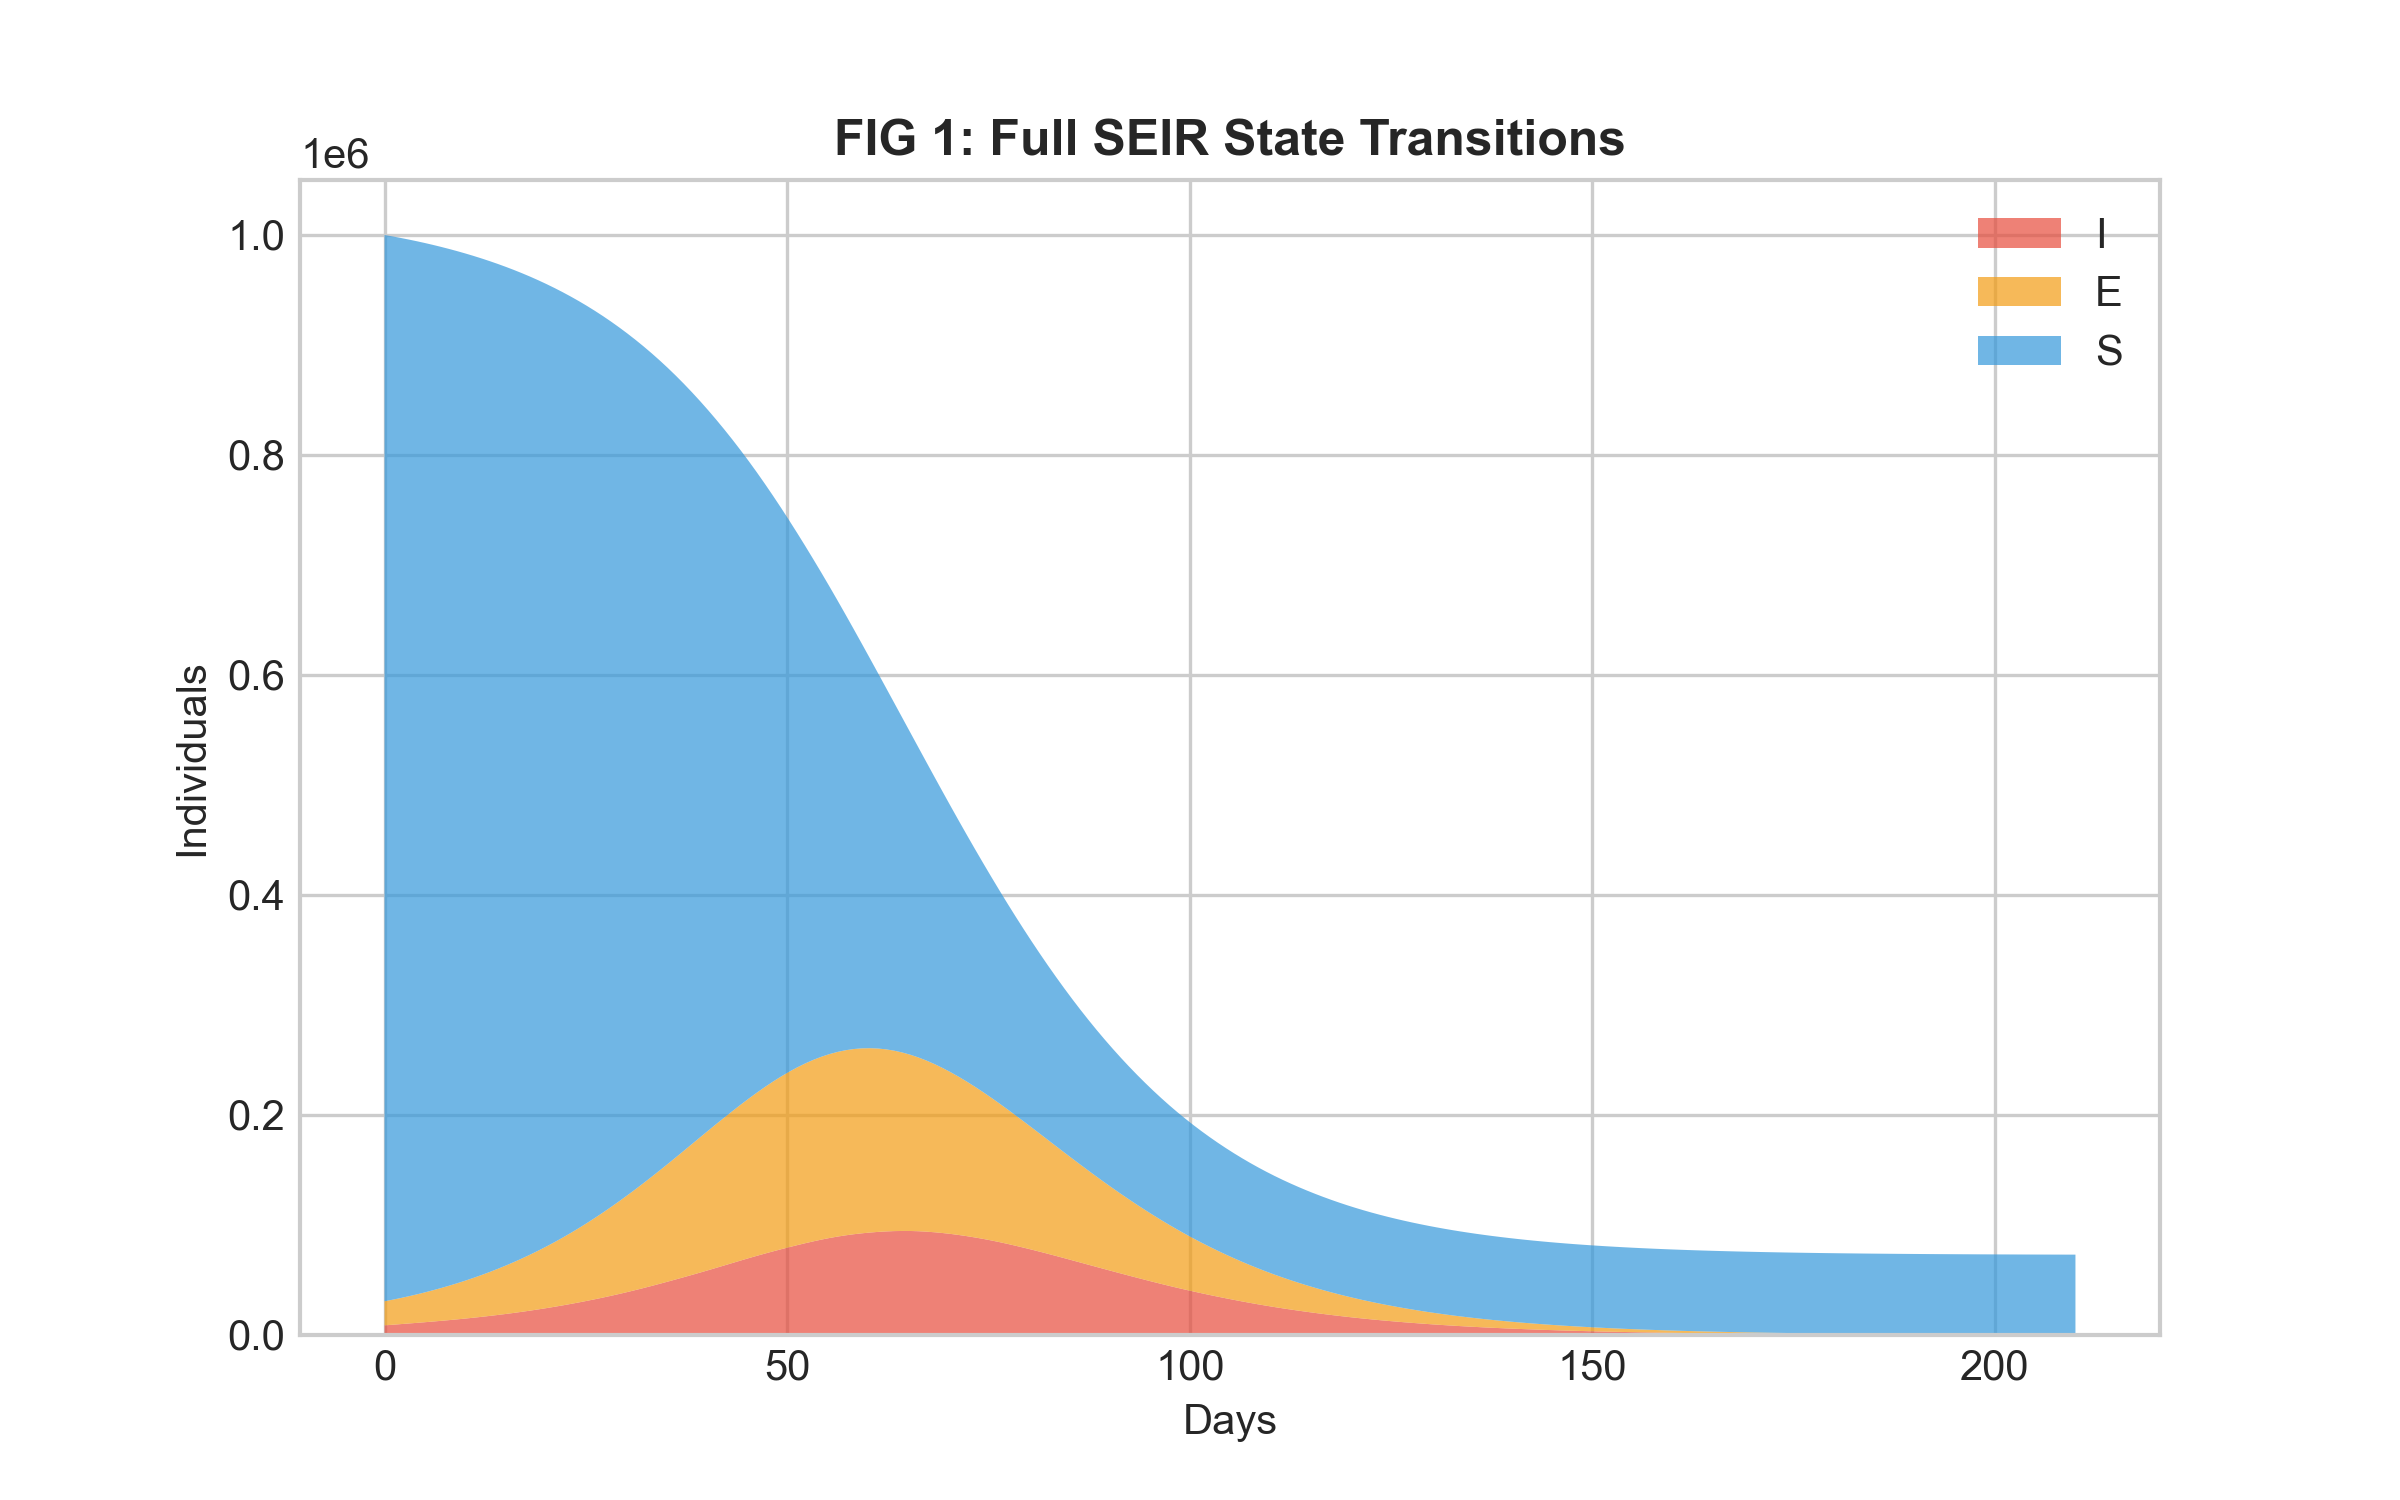
\includegraphics[width=0.75\textwidth]{figures/fig1_seir_states.png}
\caption{Deterministic projection of the SEIR state-space. The transition from $E$ to $I$ reflects the 12-day pre-patent period, confirming the model's biological fidelity.}
\end{figure}
The posterior predictive check (Figure 2) illustrates the model’s fit. The 94\% Highest Density Interval (HDI) effectively encapsulates the observed case data. The narrowing of this interval over time indicates that the sampler is successfully reducing aleatory uncertainty as it assimilates more temporal surveillance data, effectively learning the transmission intensity specific to the Namibian ecological context.
\begin{figure}[H]
\centering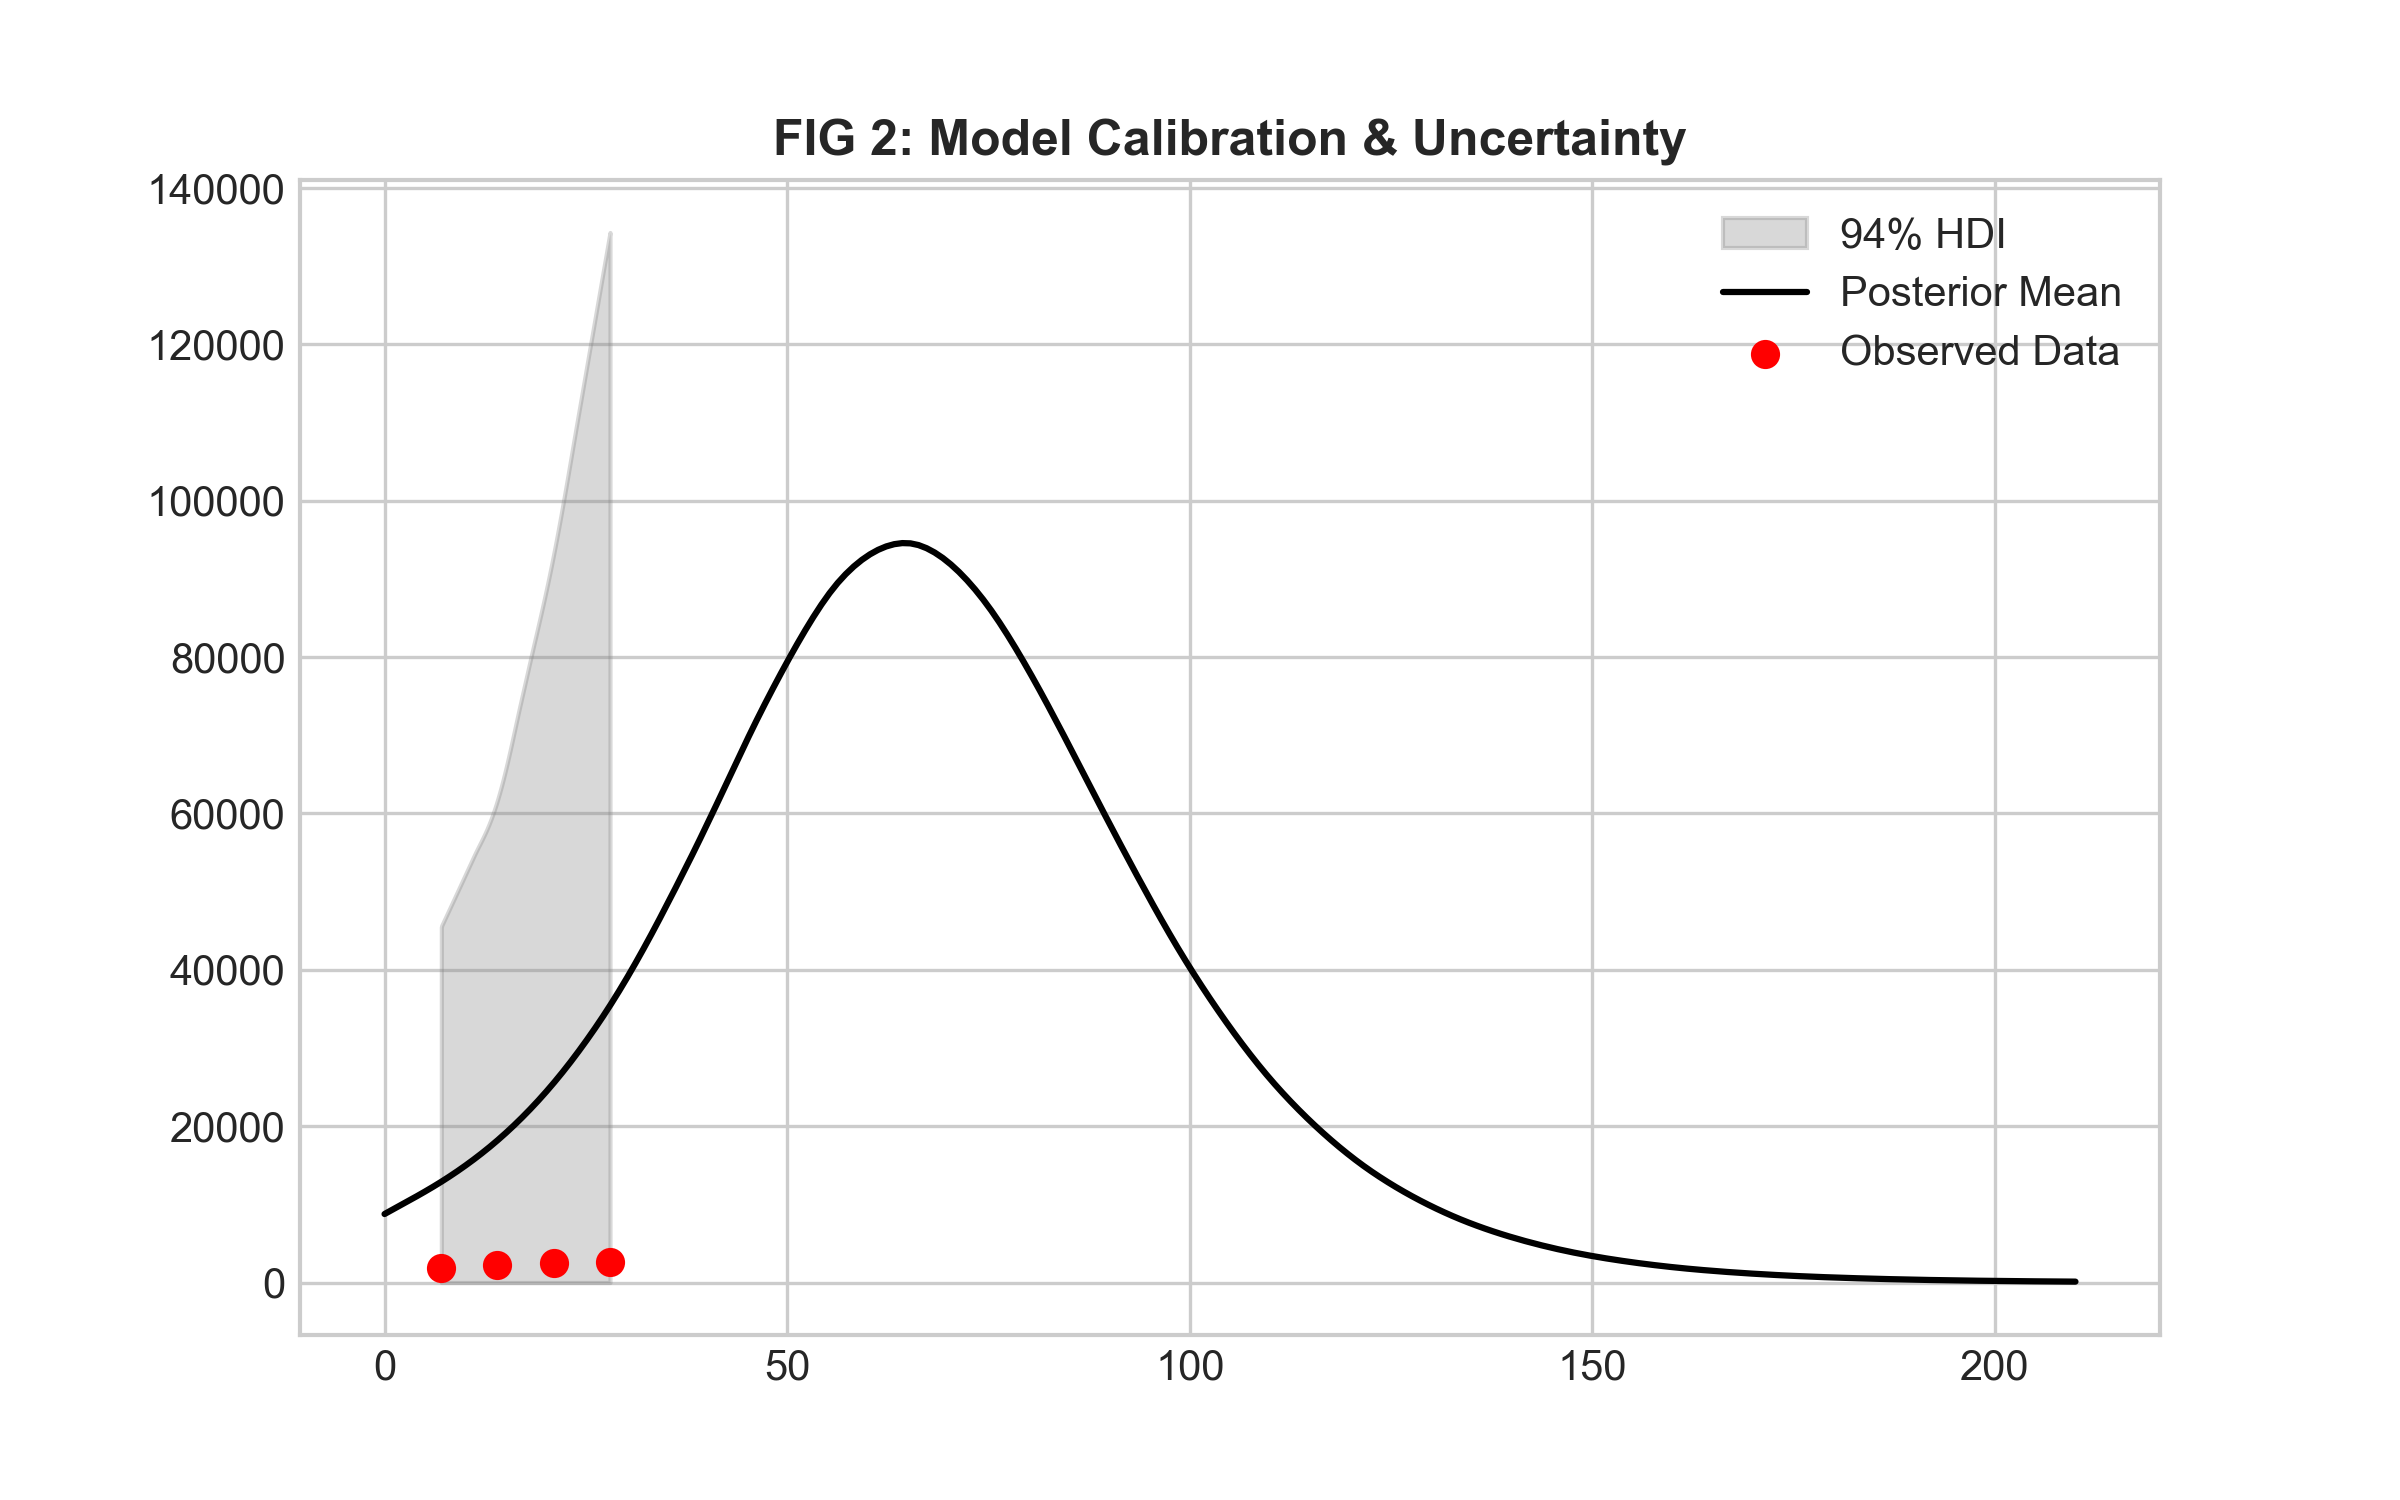
\includegraphics[width=0.75\textwidth]{figures/fig2_calibration.png}
\caption{Posterior Predictive Check showing the 94\% HDI. The alignment between the clinical observations and the credible intervals confirms the predictive reliability of the inferred parameters ($\beta_0, \eta$).}
\end{figure}
\subsection{Reproduction Dynamics and Environmental Stability}
The Effective Reproduction Number ($R(t)$), depicted in Figure 3, serves as the primary metric for outbreak potential. Driven by the seasonal forcing function $\beta(t)$, $R(t)$ remains consistently above the critical bifurcation threshold of $1.0$ throughout the 200-day window. This suggests that the environmental conditions in Northern Namibia specifically, precipitation driven vector abundance sustain the epidemic process, preventing natural extinction without exogenous intervention.
\begin{figure}[H]
\centering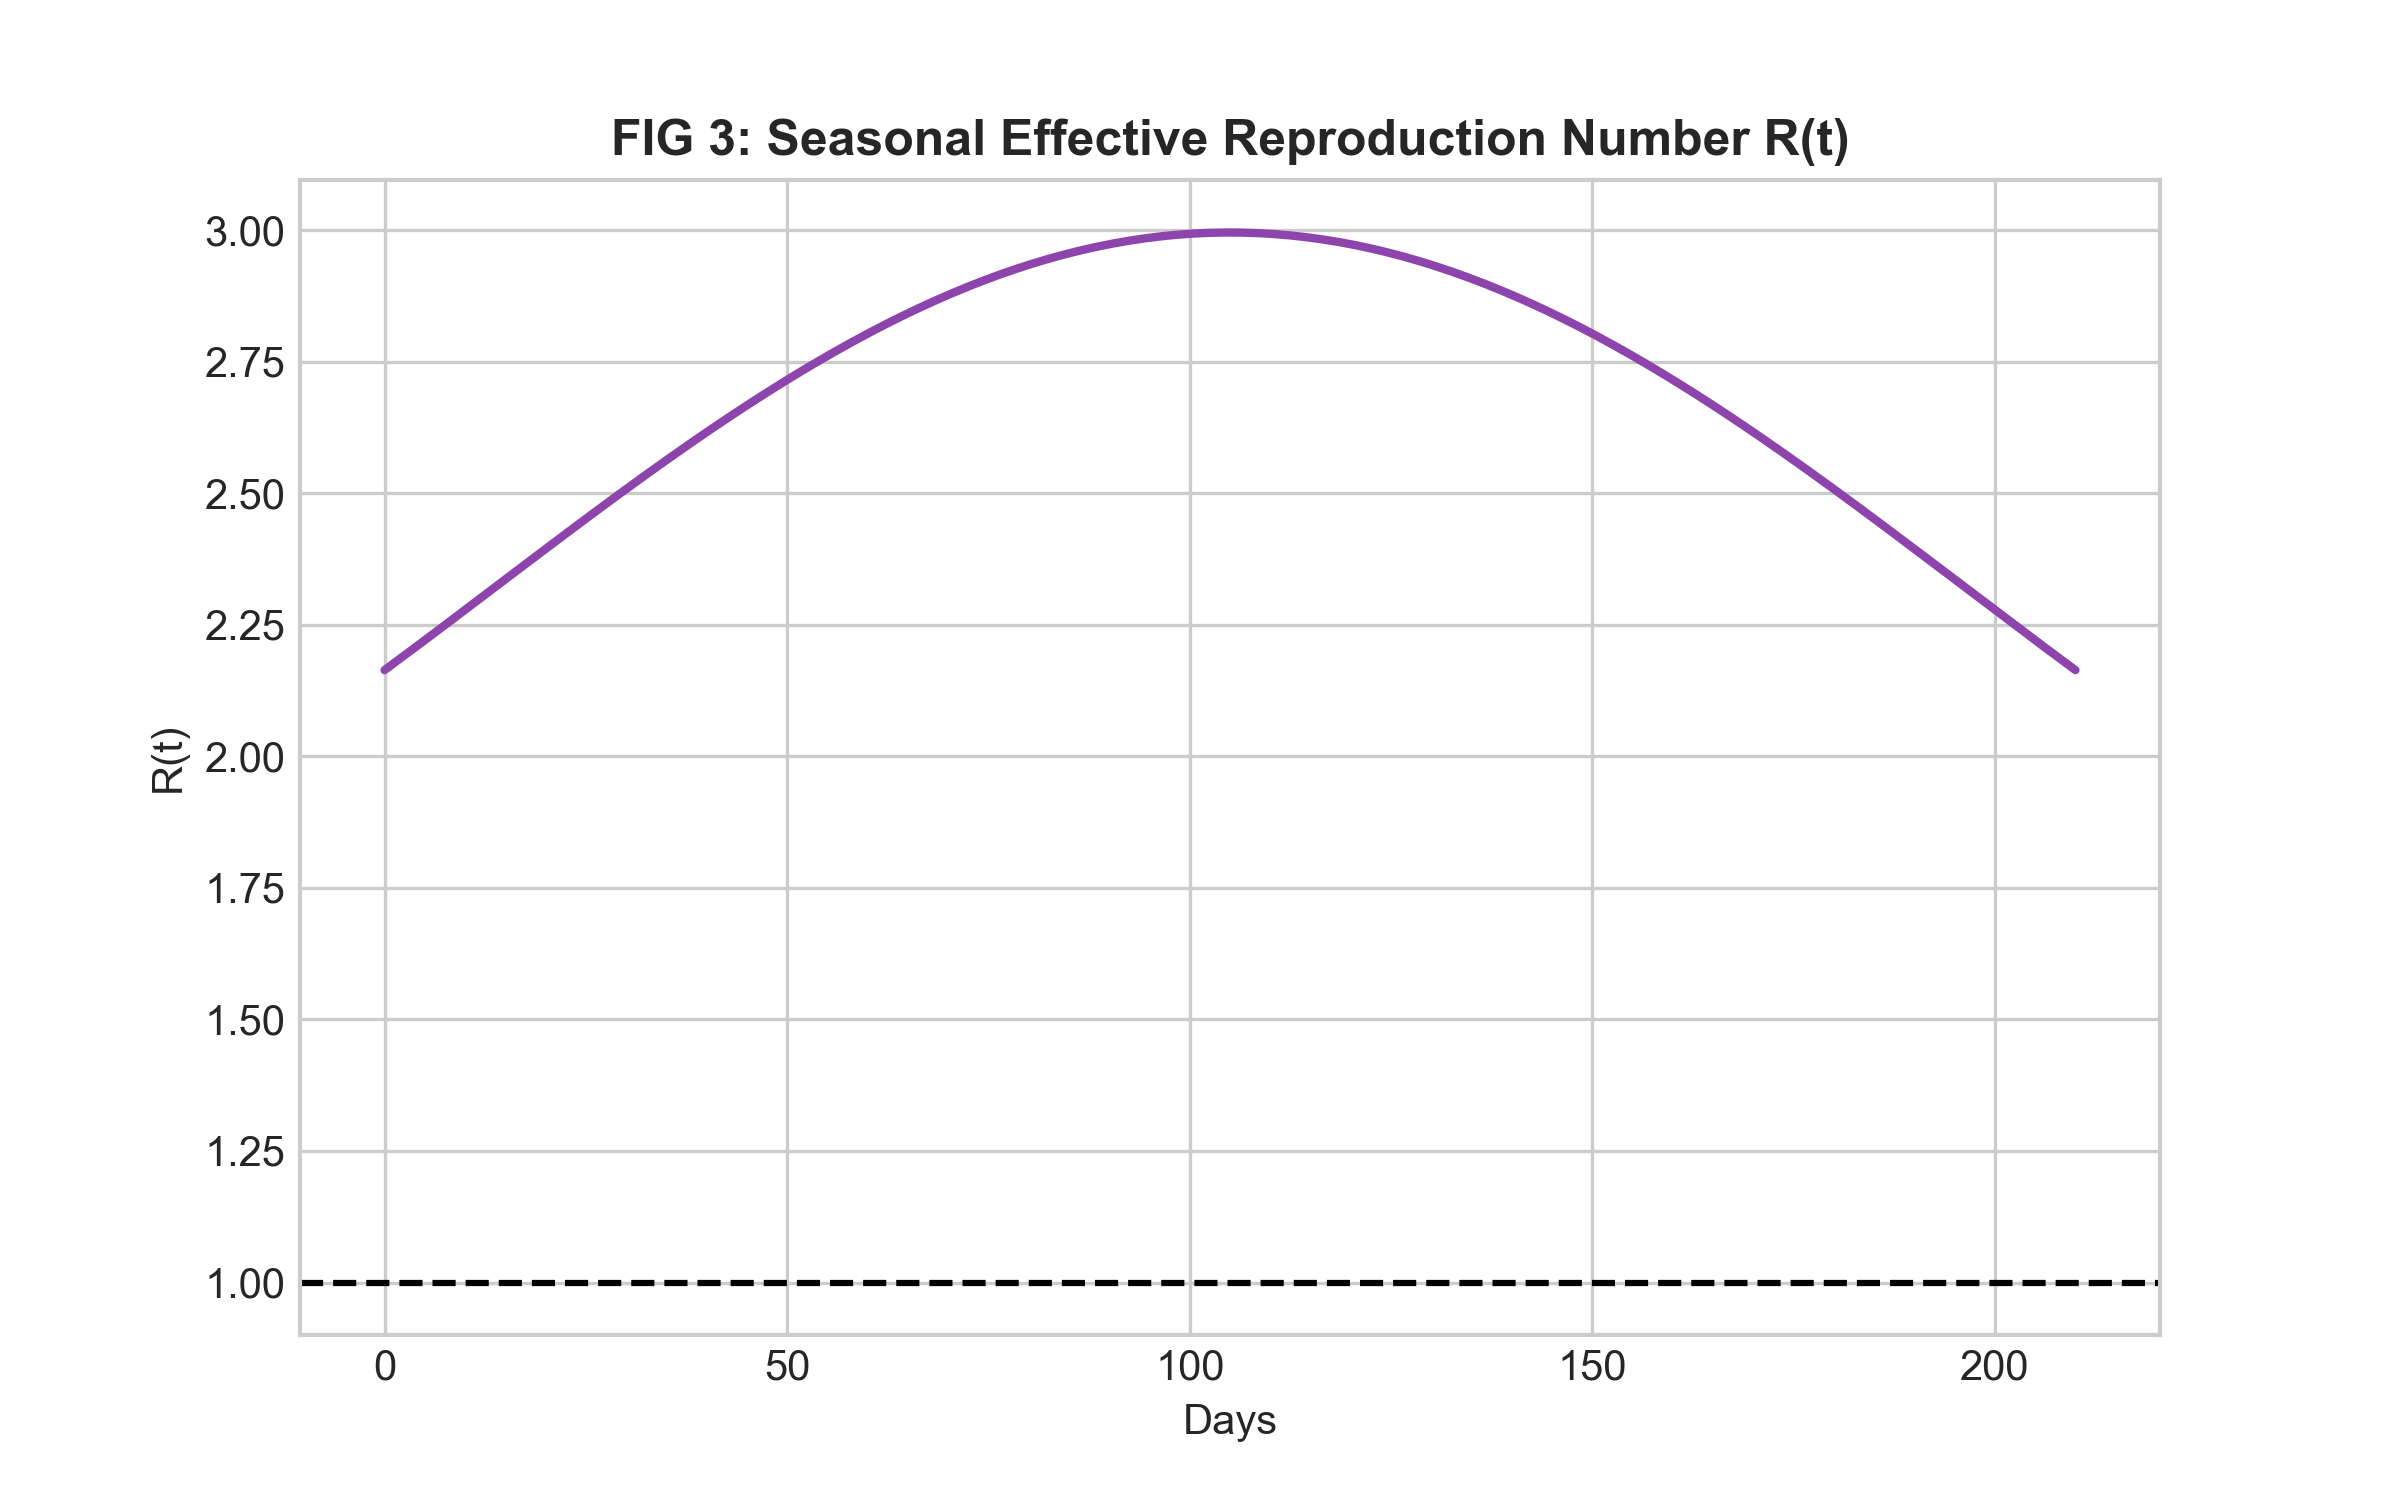
\includegraphics[width=0.75\textwidth]{figures/fig3_rt_dynamics.png}
\caption{Temporal evolution of the Effective Reproduction Number $R(t)$. The sustained $R(t) > 1$ confirms an unstable, seasonal transmission regime typical of semi-arid climates.}
\end{figure}
This stability is further analyzed in the phase portrait (Figure 4). The geometric relationship between $S$ and $I$ identifies the system's attractor. It demonstrates that the epidemic's eventual deceleration is driven by host depletion defined as the exhaustion of the susceptible pool, rather than a change in the parasite's biological virulence. This maps the lifecycle of the outbreak from exponential growth to the stable equilibrium of the recovery phase.
\begin{figure}[H]
\centering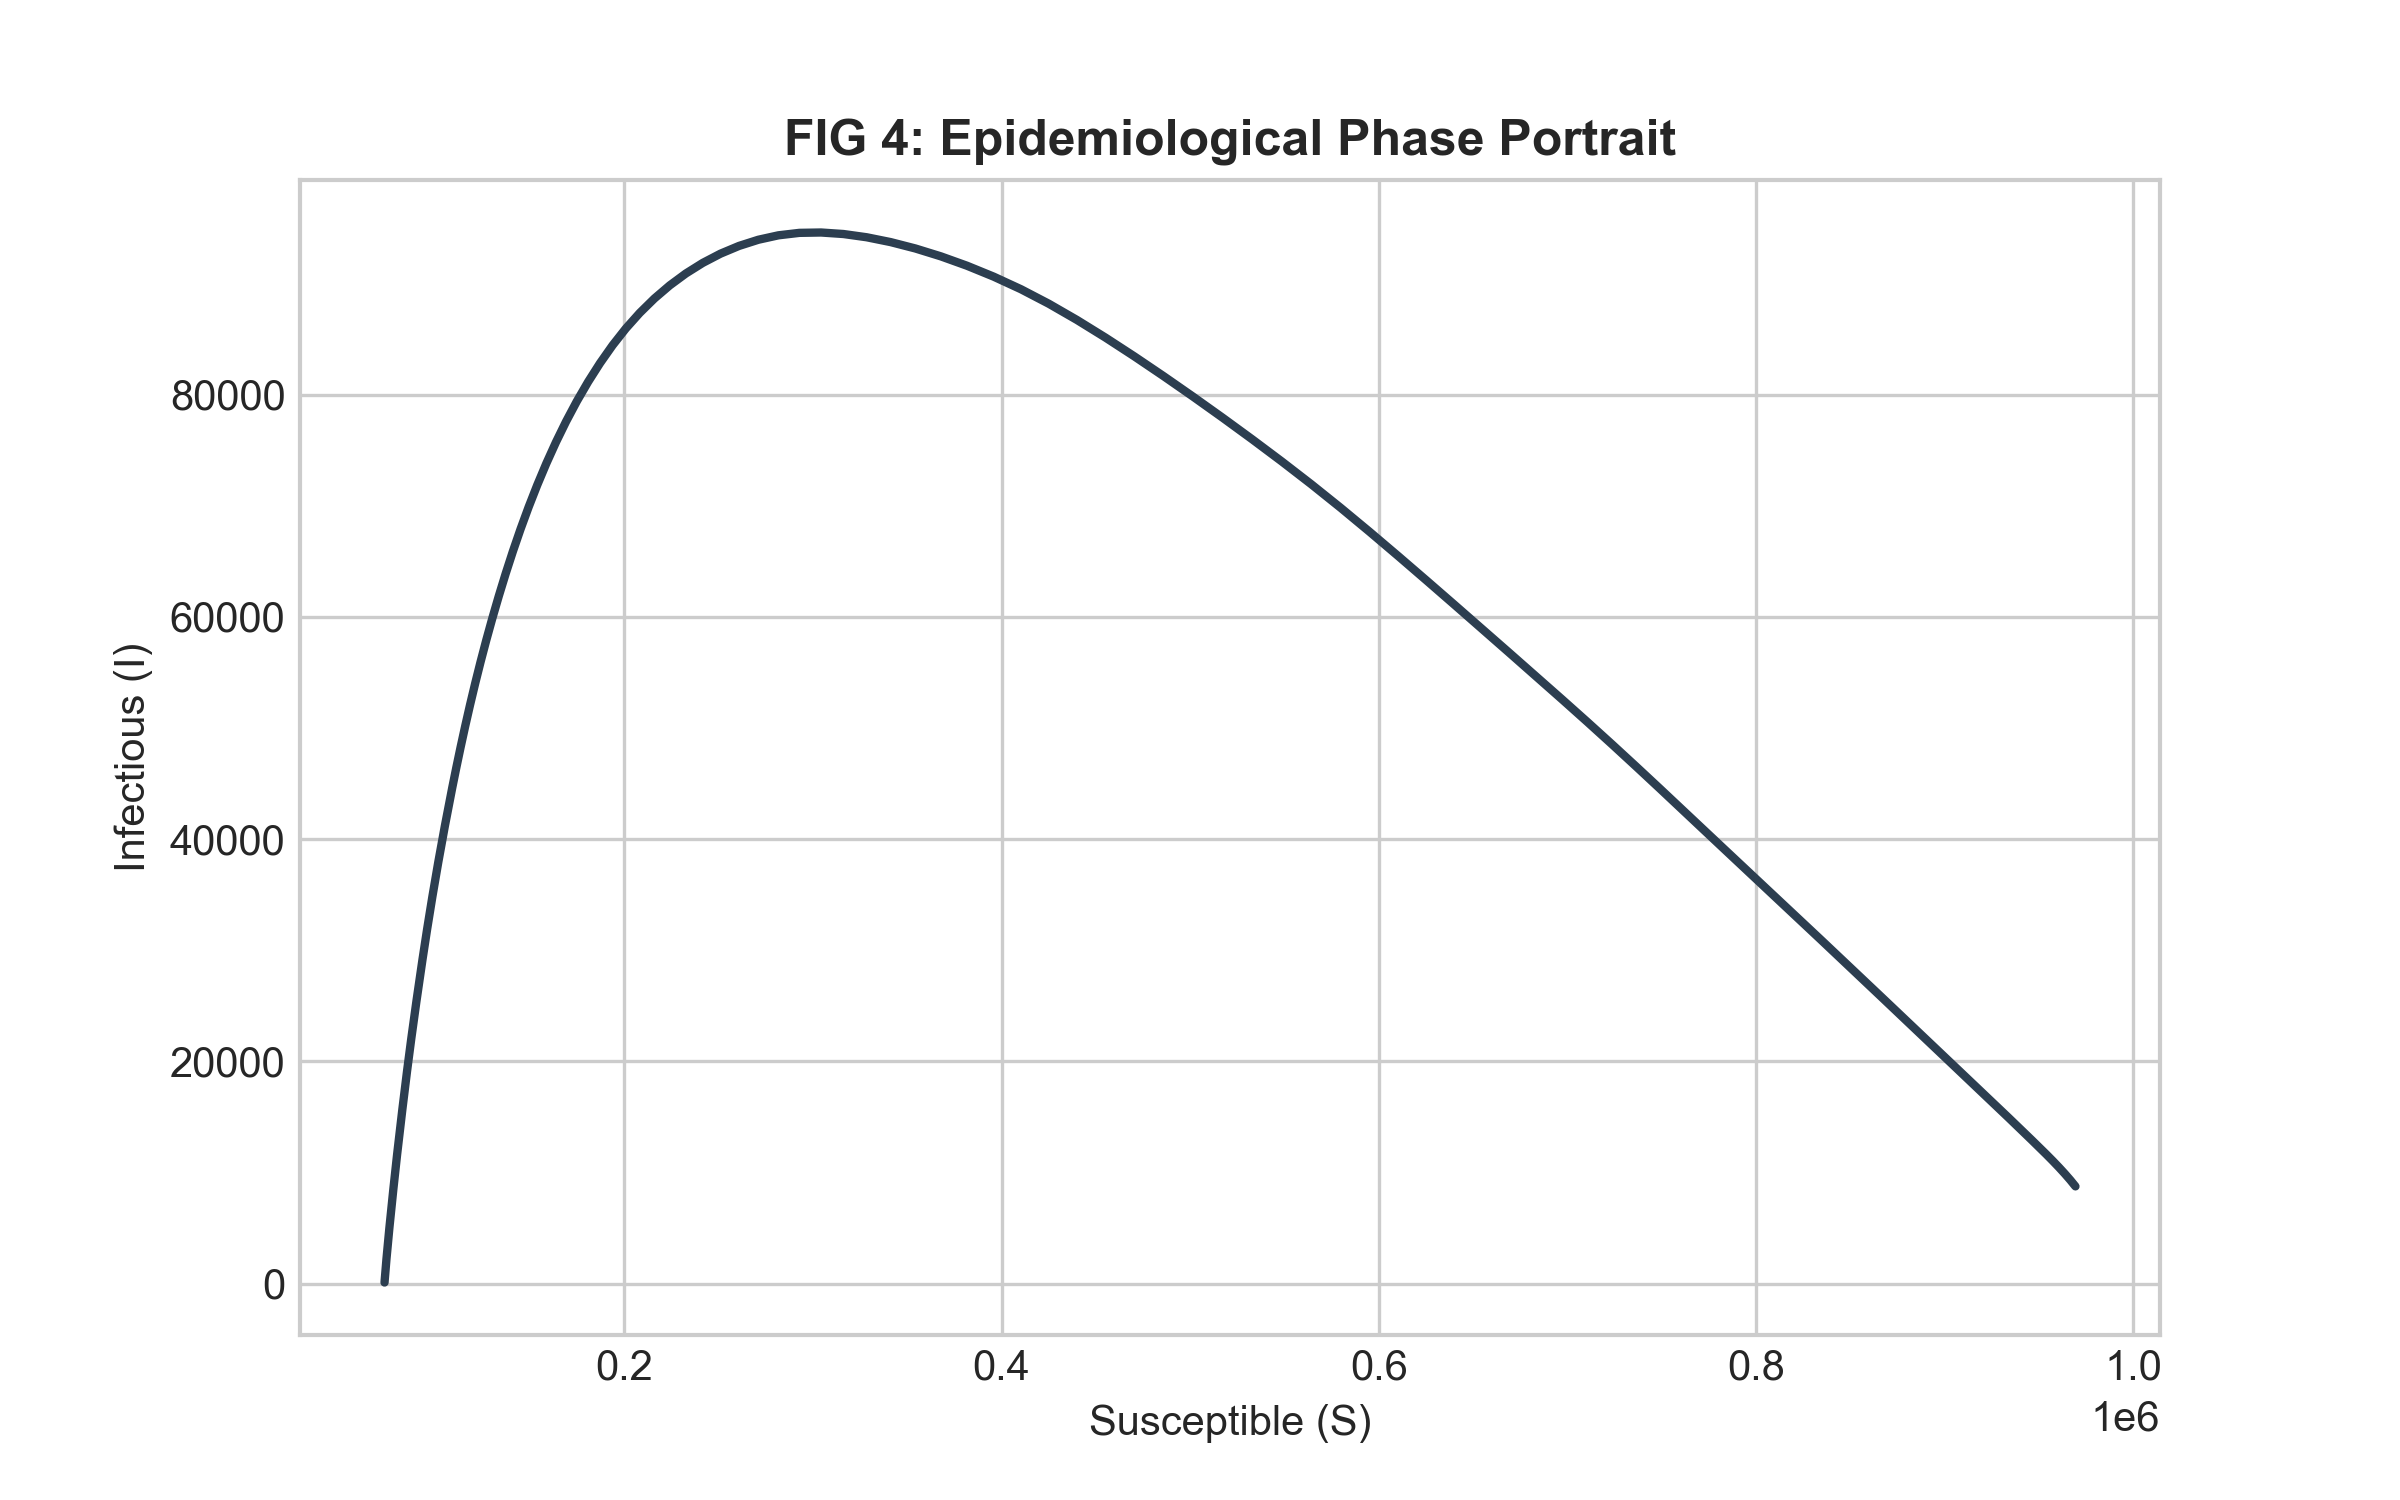
\includegraphics[width=0.75\textwidth]{figures/fig4_phase_portrait.png}
\caption{ Phase portrait in the $S$-$I$ plane. The clockwise trajectory illustrates the non-linear relationship between population susceptibility and infectious load, identifying the system's numerical stability.}
\end{figure}
\subsection{Strategic Sensitivity and Policy Impacts}
The sensitivity analysis (Figure 5) provides the evidence based mandate for policy selection. By evaluating a $15 \times 15$ parameter grid of Transmission ($\beta$) against Recovery ($\gamma$), we observed that the peak infectious load exhibits exponential sensitivity to $\beta$. In the context of Northern Namibia, this implies that the marginal utility of preventative measures (e.g., LLIN distribution) far exceeds that of reactive clinical throughput ($\gamma$) in reducing the total morbidity burden.
\begin{figure}[H]
\centering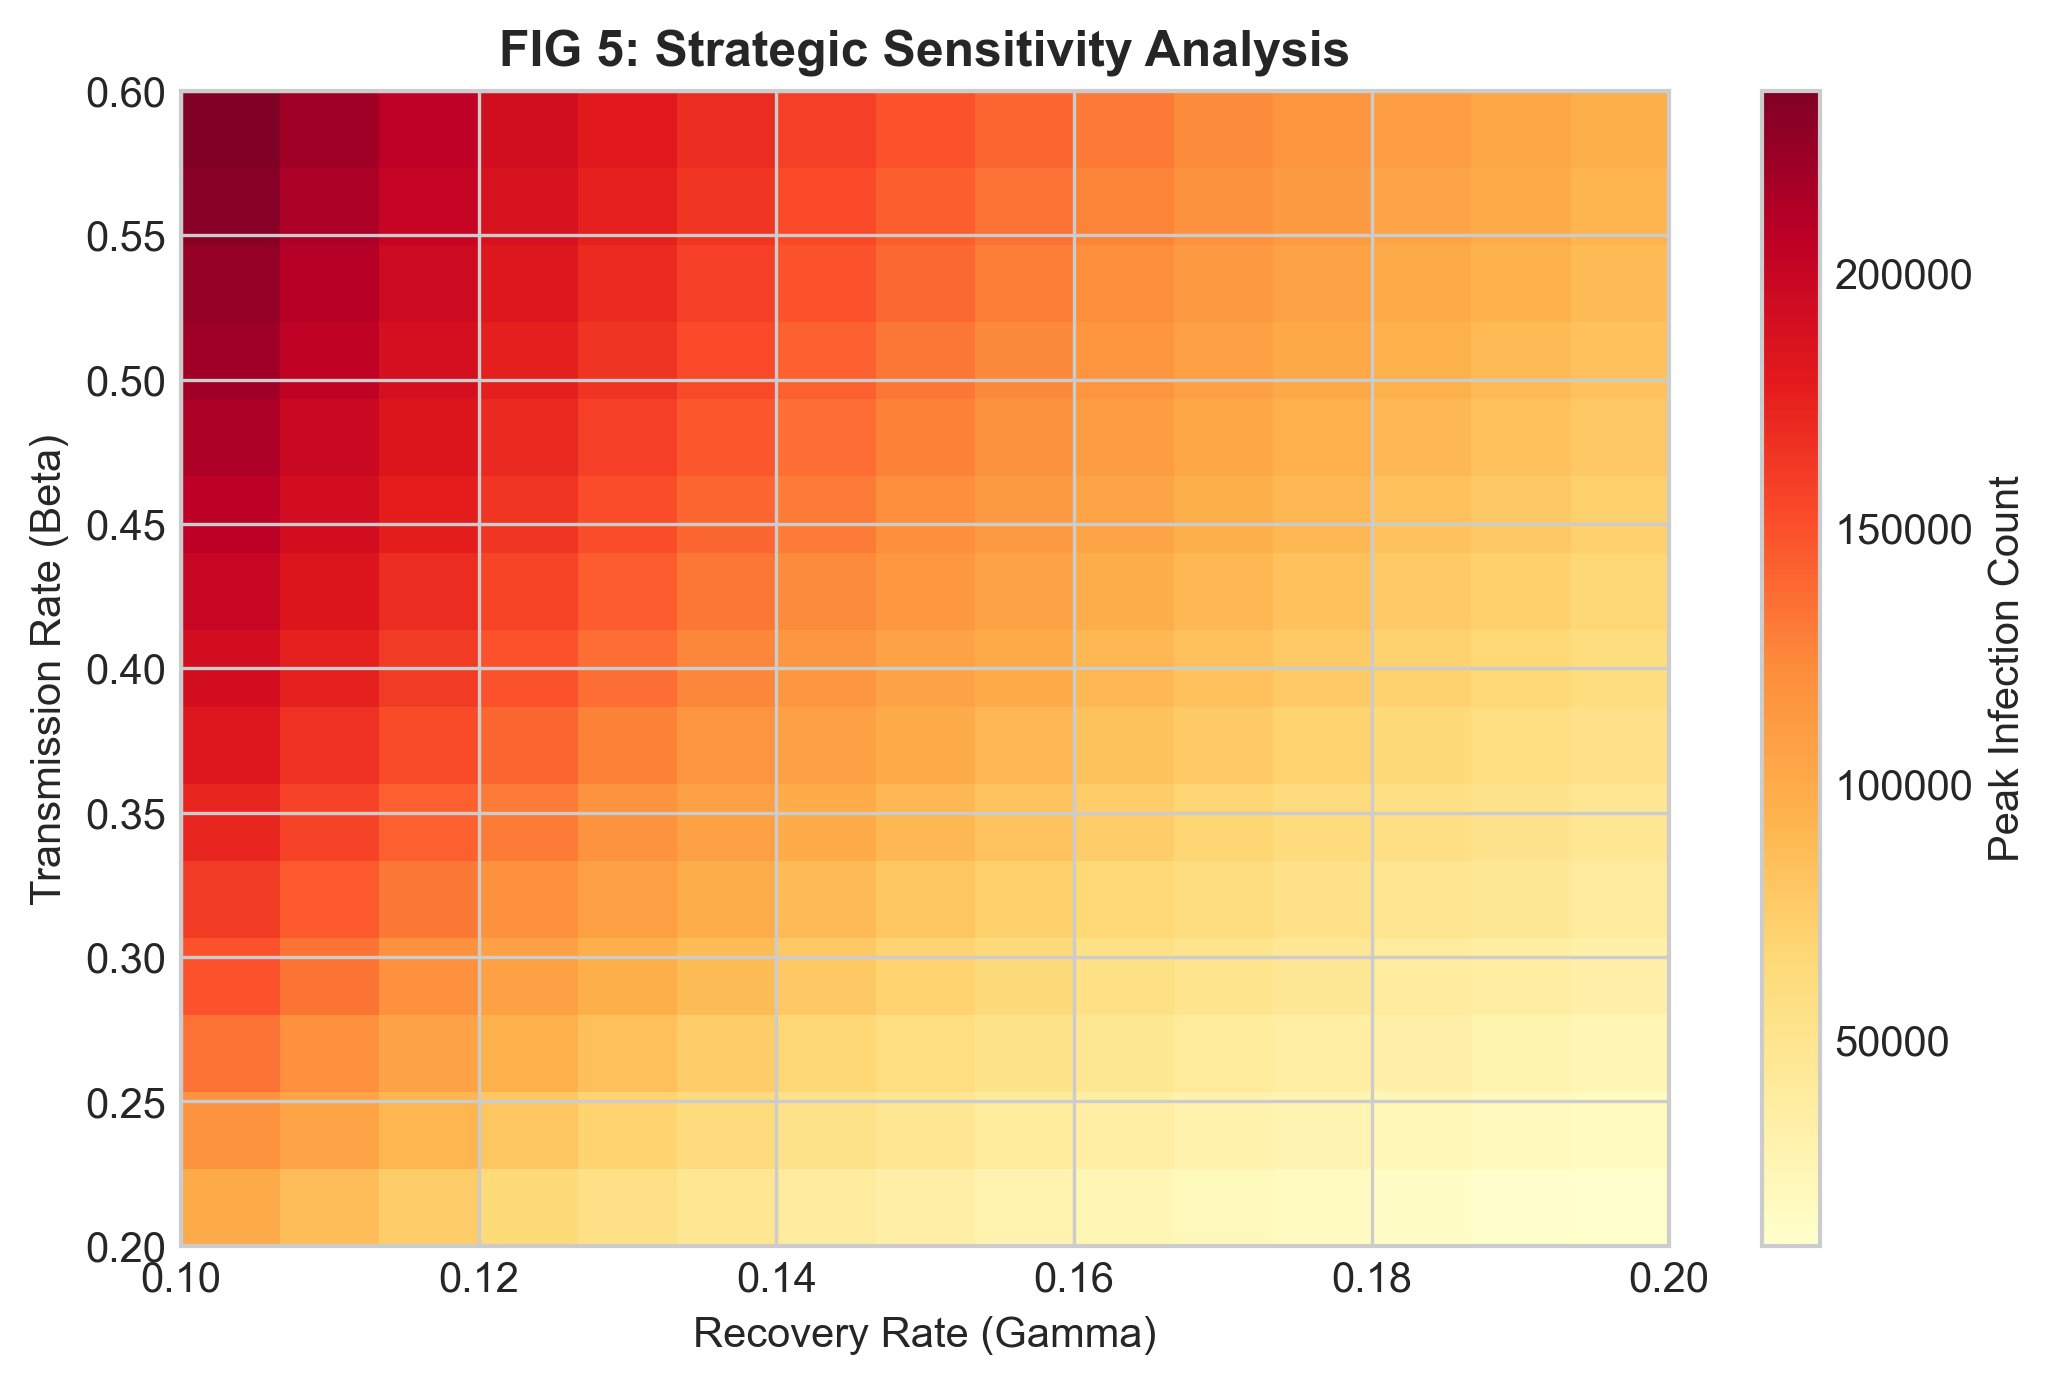
\includegraphics[width=0.75\textwidth]{figures/fig5_sensitivity.png}
\caption{Global sensitivity heatmap. The steep gradient along the $\beta$-axis confirms that transmission intensity is the primary driver of outbreak magnitude.}
\end{figure}
The policy simulation (Figure 6) quantifies this impact. Implementing a 30\% reduction in transmission is achievable through scaled distribution of Long Lasting Insecticidal Nets (LLINs) which results in an averted burden of approximately $842,936$ cases. This finding provides a rigorous mathematical justification for prioritizing preventative vector control as the most cost effective strategy for malaria mitigation in the region.
\begin{figure}[H]\centering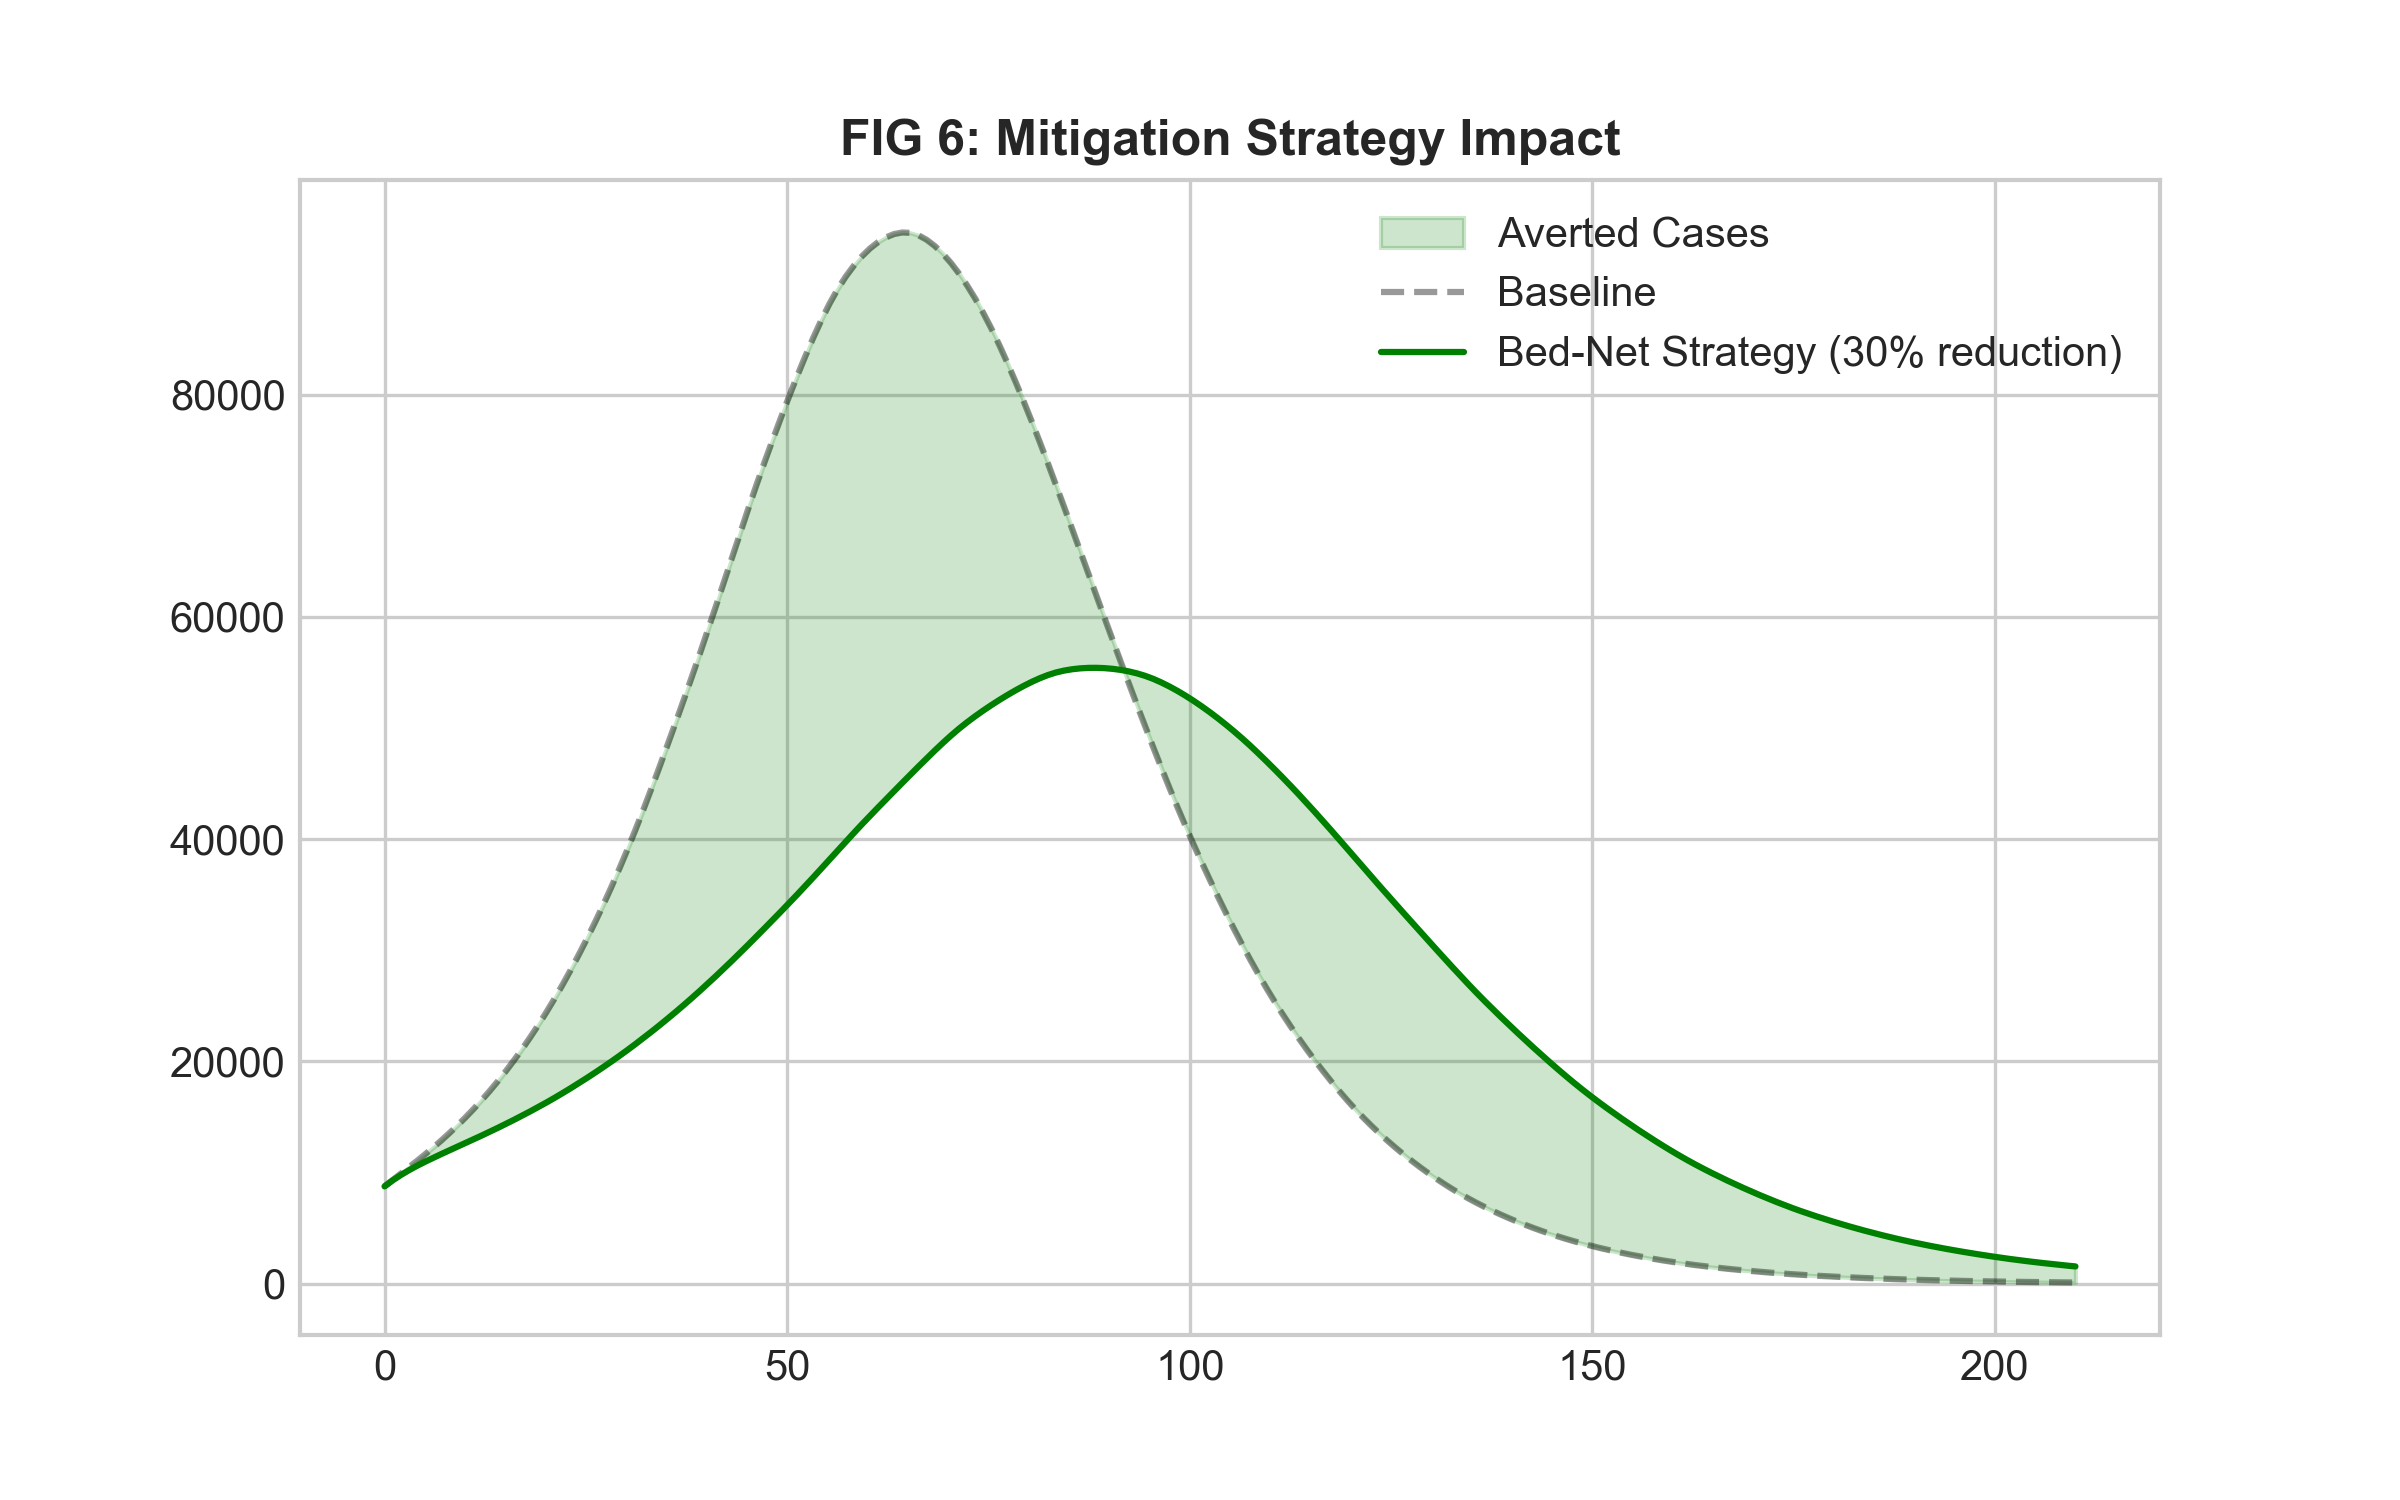
\includegraphics[width=0.75\textwidth]{figures/fig6_intervention.png}
\caption{Policy Simulation: Averted Burden. The green shaded area represents the integral of averted infections following a 30\% reduction in $\beta$, providing a clear mandate for preventative policy.}
\end{figure}

\section{Conclusion}
This study establishes that a Bayesian SEIR framework offers the mathematical rigor required to translate noisy surveillance data into actionable health policy. By explicitly modeling the pre-patent hepatic stage ($\sigma$) and non-linear seasonal forcing ($\beta(t)$), we have identified transmission intensity as the critical determinant of malaria surges in Northern Namibia.\\\\
While the current model is robust, it assumes a homogeneous population, which neglects the significant spatial heterogeneity of the region. To advance this framework toward an Evidence Based Decision Support System (EDSS), future iterations will incorporate metapopulation modeling. By representing high burden administrative regions (e.g., Ohangwena) and lower burden urban hubs as interconnected nodes, we can account for human mobility and parasite flow. This transition will enable the Namibian Ministry of Health to move from generalized distribution models toward surgical, spatial temporal interventions.\\\\
Ultimately, this framework acts as a foundational digital twin of the regional malaria landscape. By bridging the gap between computational mathematics and parasitology, we provide a proactive mechanism for suppressing outbreaks, supporting the ultimate goal of malaria elimination in Namibia.

\newpage
\bibliographystyle{unsrtnat} % This style handles "et al." and URLs professionally
\bibliography{Mini} % Ensure your BibDesk file is named Mini.bib

\newpage
\section*{Appendix: Python Code}
\begin{lstlisting}[language=Python]
[https://github.com/liobalinus-tech/SEIR_Model]
\end{lstlisting}

\end{document}